\begin{frame}
	\centering
	\begin{tikzpicture}
		\path[use as bounding box] (-6,0) -- (2,0);
		\node at (0,0) {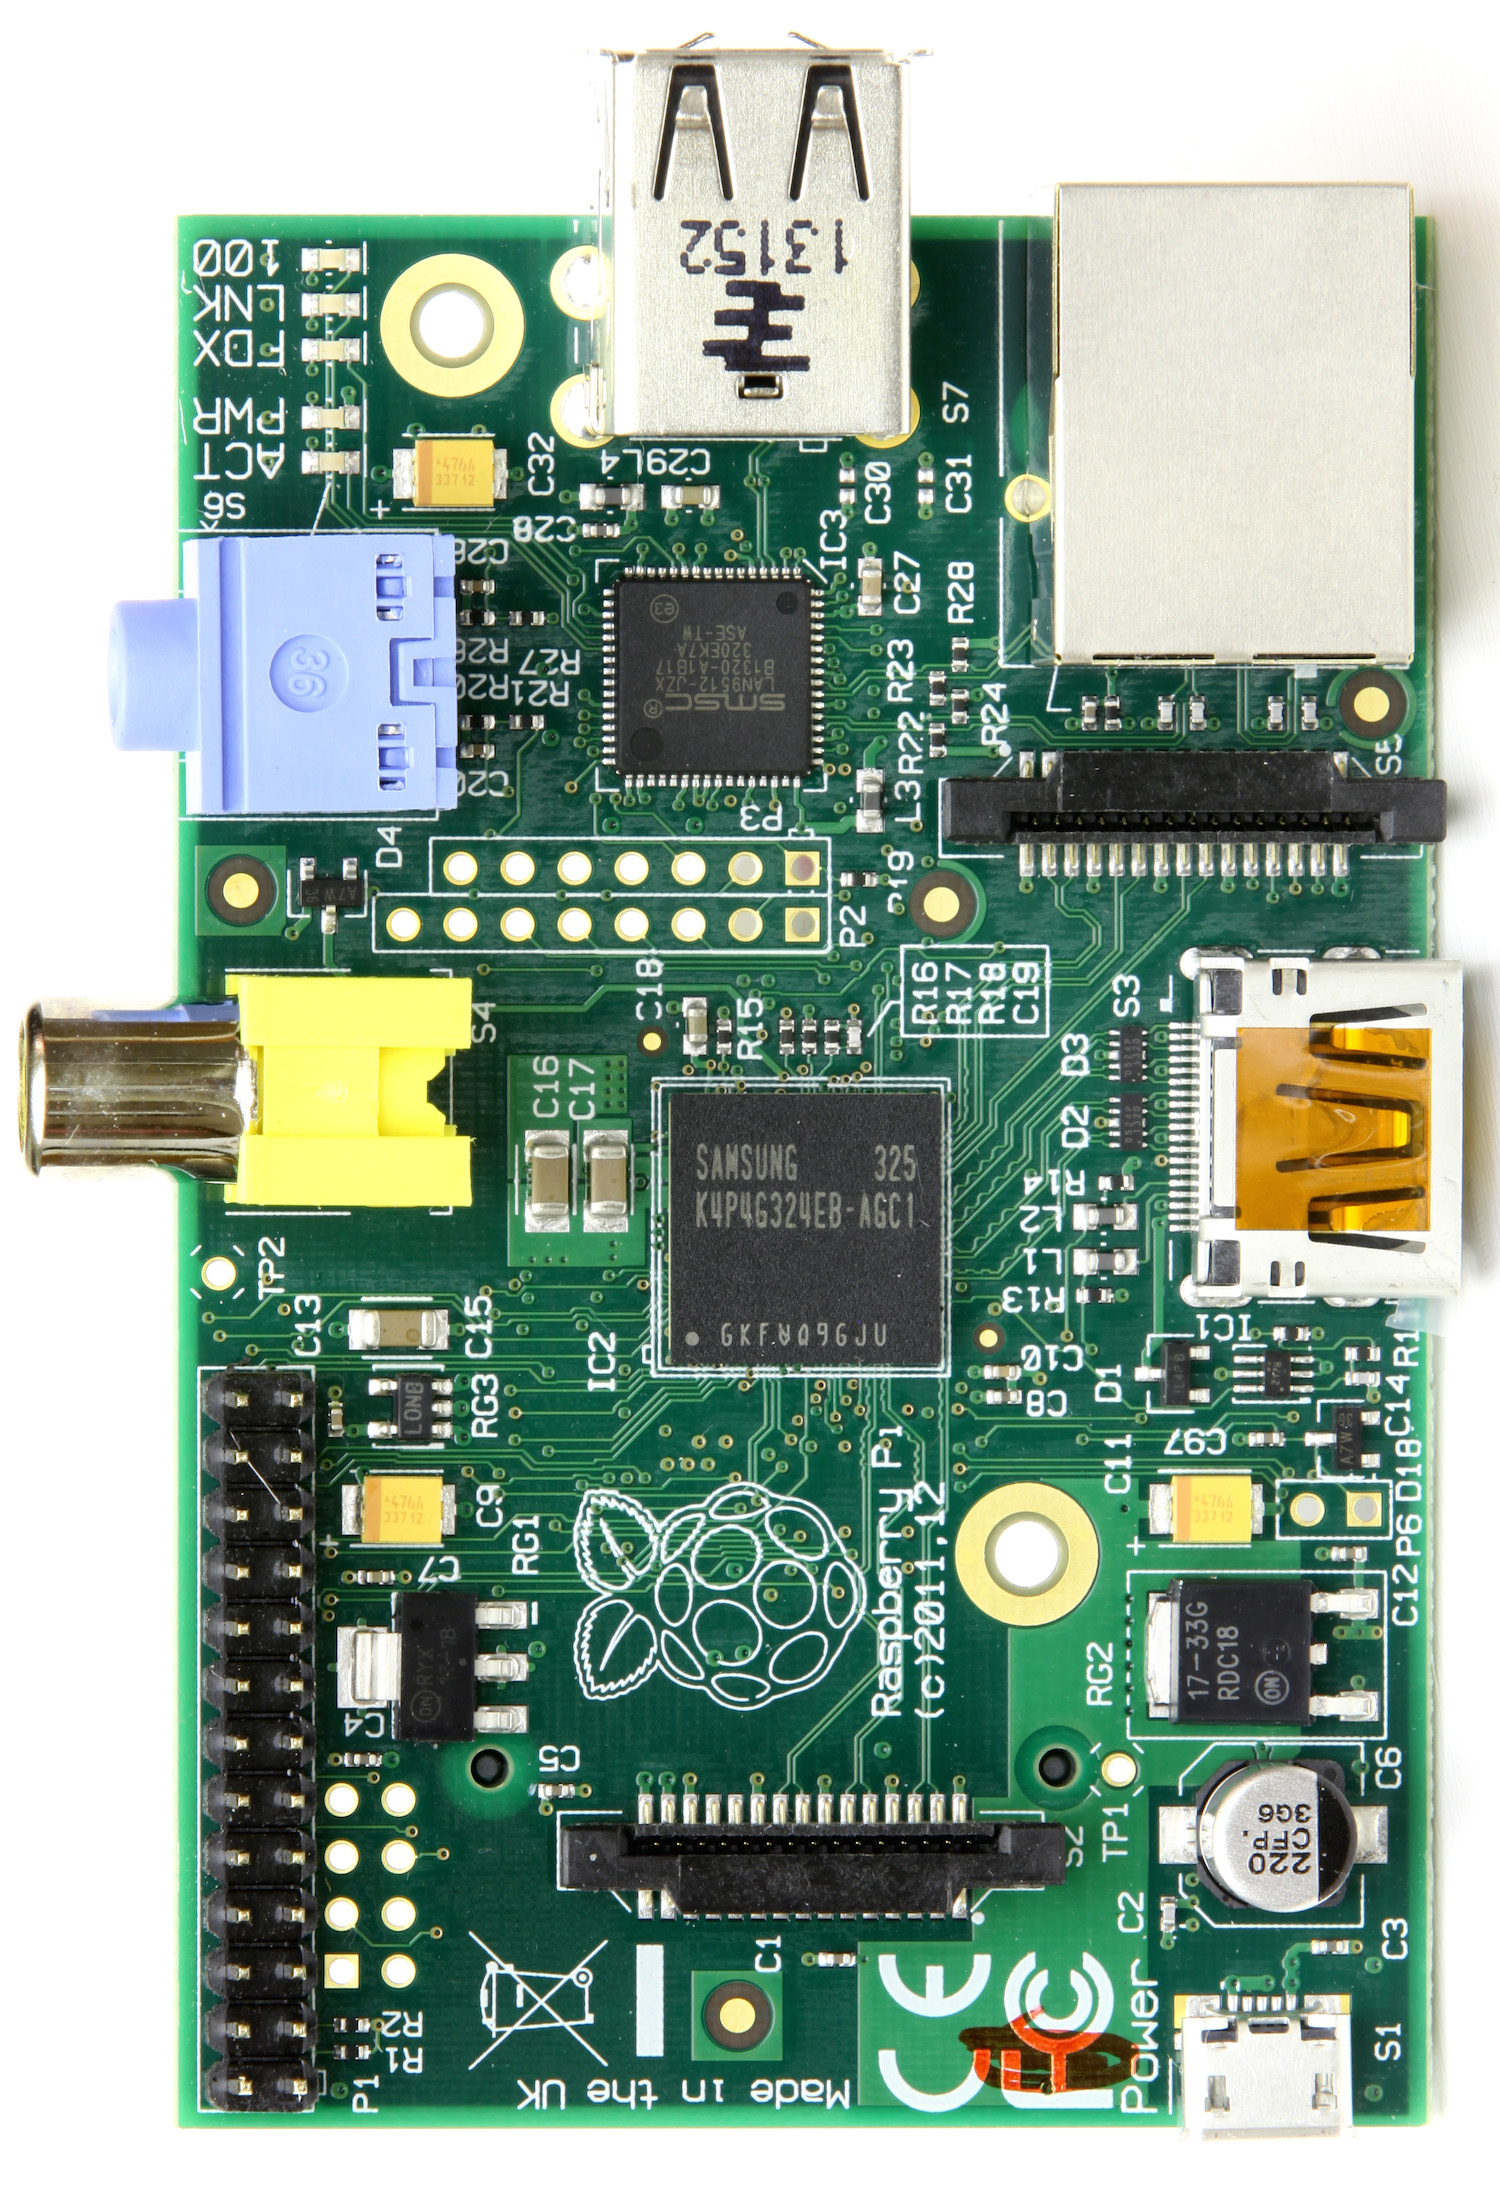
\includegraphics[width=3cm]{img/raspi.jpg}};
		\pause
		\node at (-2.8,-2.1) {
\includegraphics[width=4cm]{img/music.png}};
		\pause
		\path[snake=expanding waves,segment length=2mm,segment angle=30,draw,thick,color=blue] (-1.3,0.85) -- +(-2,0);
	\end{tikzpicture}
\end{frame}

\begin{frame}
	\frametitle{GPIO Keyboard}
	\centering
	\begin{tikzpicture}
		\node at (-4,2) {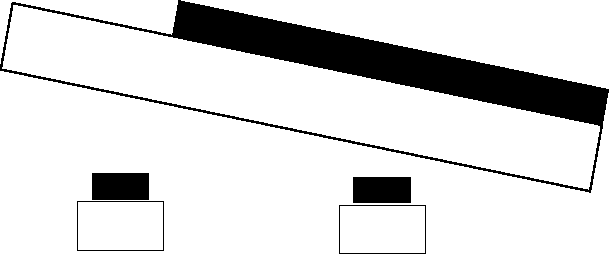
\includegraphics[width=4cm]{img/key1.pdf}};
		\node[align=left ,text width=4cm] at (1,2) { Two buttons connected \\ to GPIO ports};
		\node at (-4,0) {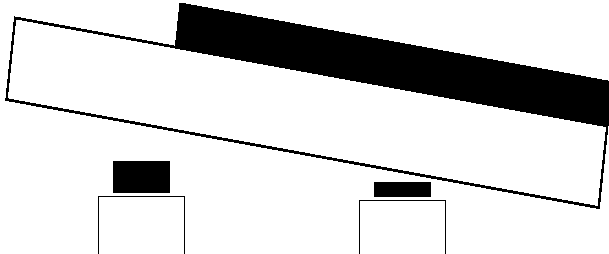
\includegraphics[width=4cm ]{img/key2.pdf}};
		\node[align=left ,text width=4cm] at (1,0) { Interrupt Time A};
		\node at (-4,-2) {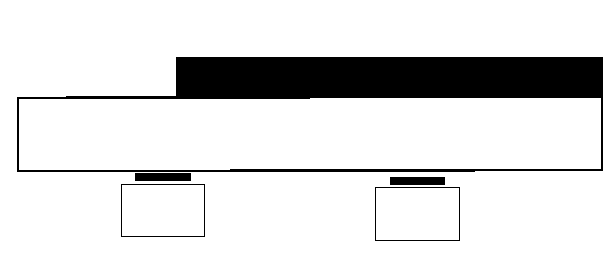
\includegraphics[width=4cm]{img/key3.pdf}};
		\node[align=left ,text width=4cm] at (1,-2) { Interrupt Time B};
		\node[align=left ,text width=6cm] at (-1,-3.5) {  $midi\_velocity=\frac{idle\_stroke}{Time B - Time A}$};
	\end{tikzpicture}	
	
\end{frame}


{
    \usebackgroundtemplate{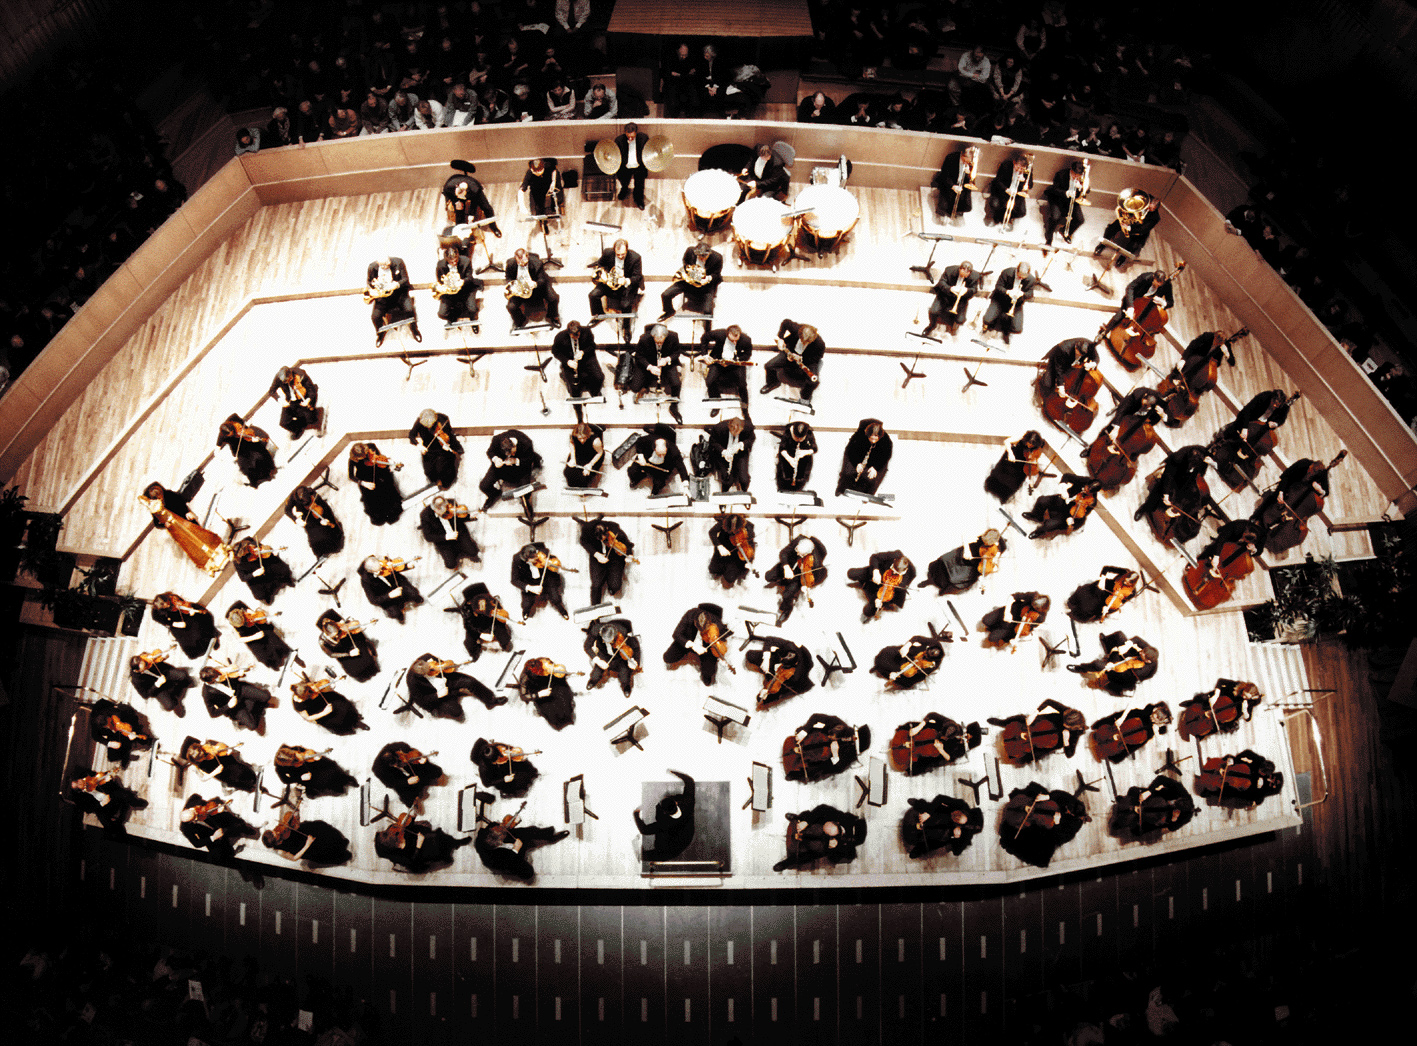
\includegraphics[height=\paperheight]{img/orchestra.jpg}}
    \setbeamertemplate{navigation symbols}{}
    \begin{frame}[plain]
    \end{frame}
}
{
    \usebackgroundtemplate{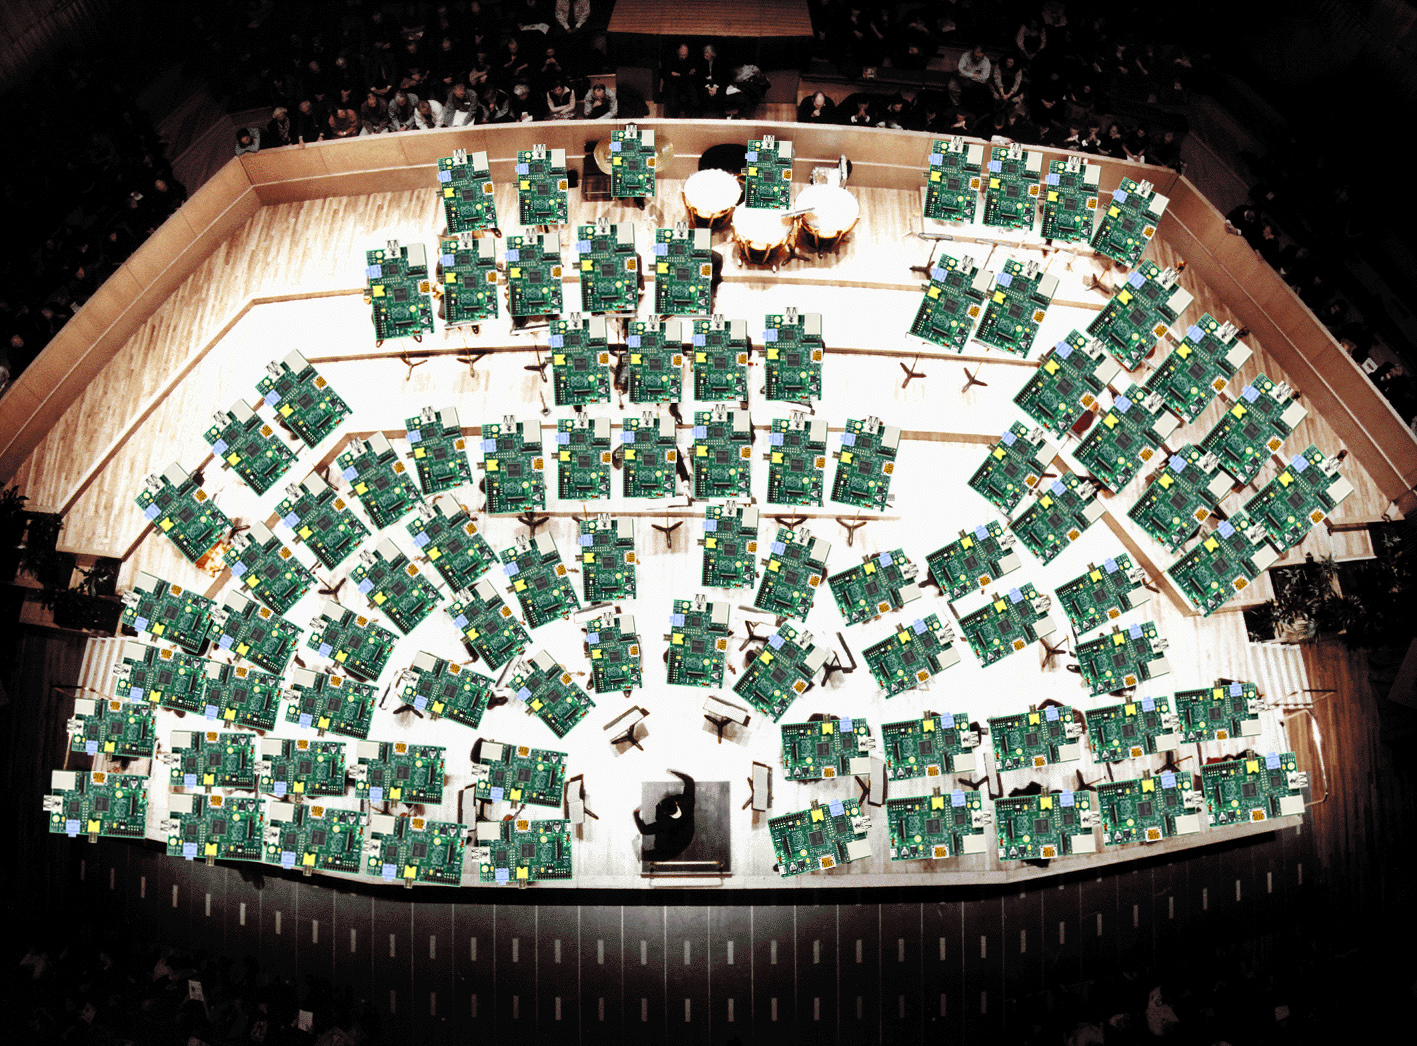
\includegraphics[height=\paperheight]{img/piorchestra.jpg}}
    \setbeamertemplate{navigation symbols}{}
    \begin{frame}[plain]
    \end{frame}
}
\begin{frame}{Composer}
	\centering
	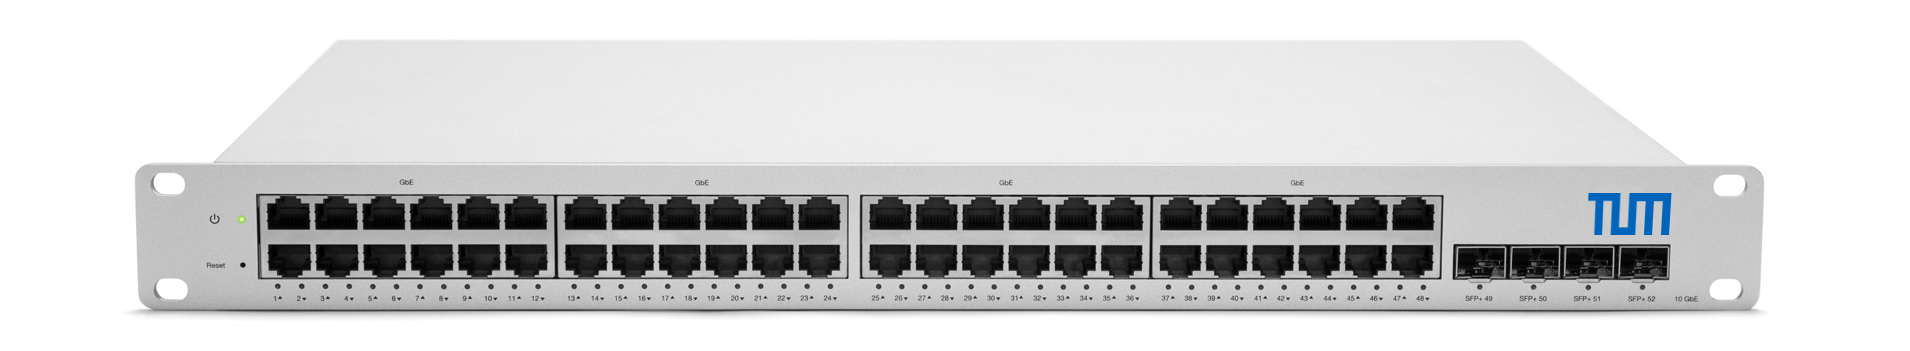
\includegraphics[width=10cm]{img/switch-raw.jpg}
\end{frame}

\begin{frame}
	\centering
	\begin{tikzpicture}
		\node at (0,-1.2) {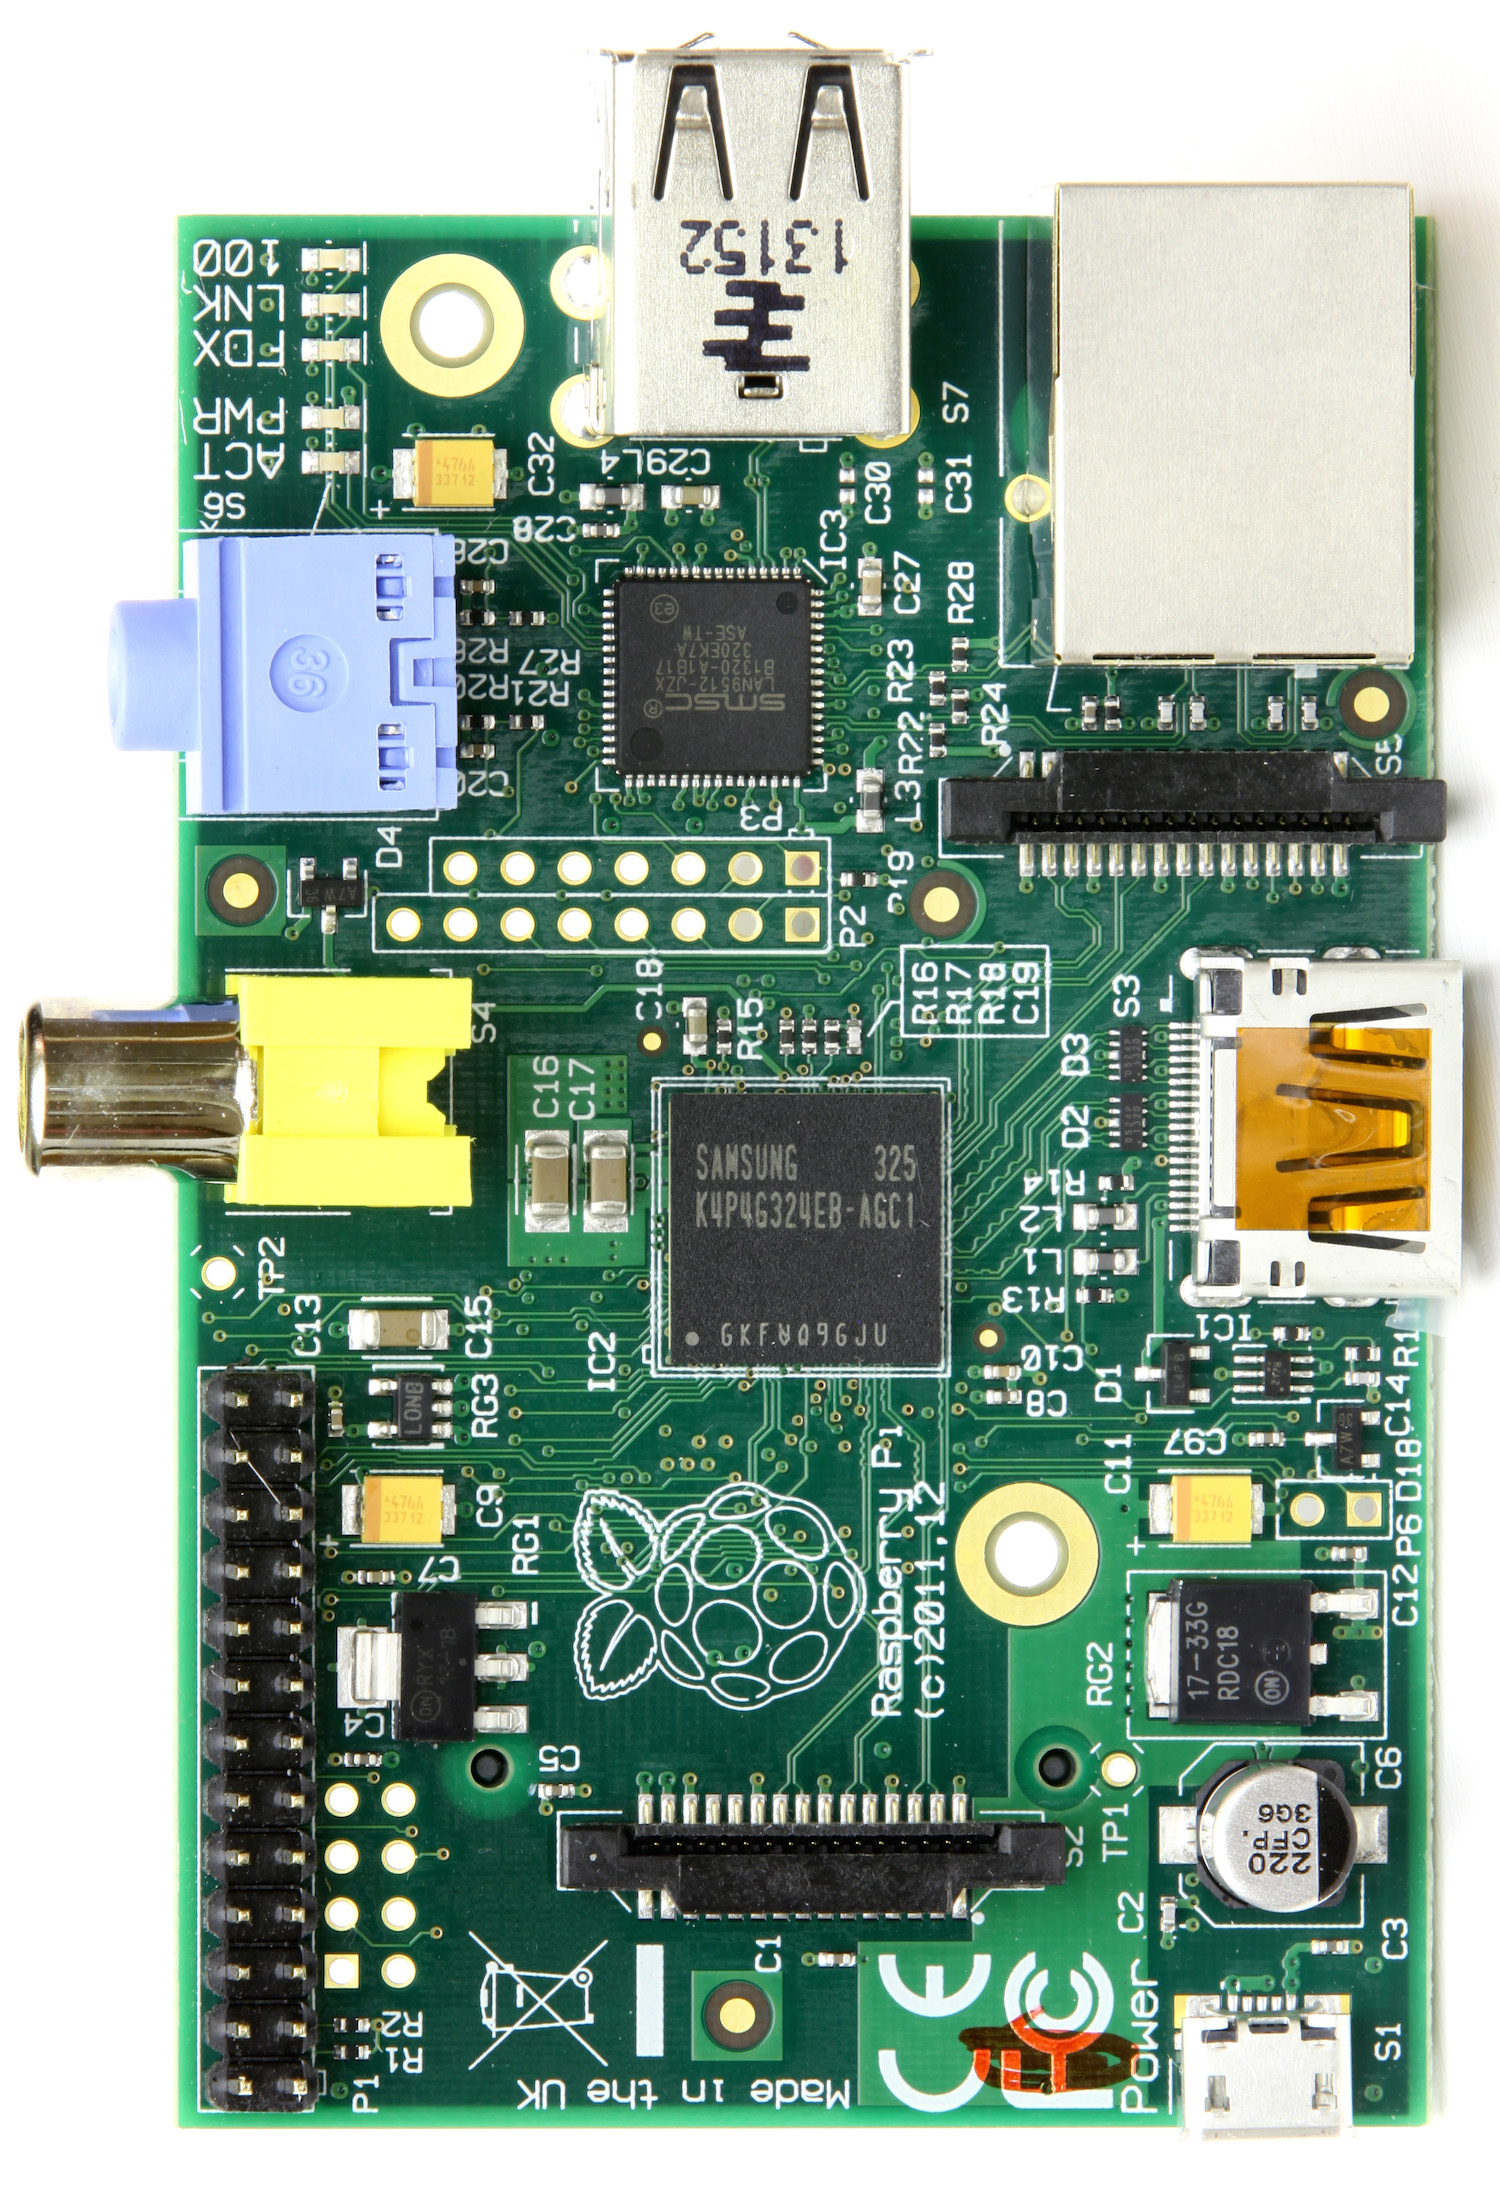
\includegraphics[width=3cm]{img/raspi.png}};
		\node at (-2.8,-3.3) {
\includegraphics[width=4cm]{img/music.png}};
		\pause
		\draw[line width=0.6em,color=blue] (1,1.8) .. controls (1,3) and(4,3) .. (4,1.8);
		\node[below] at (3.97,2) {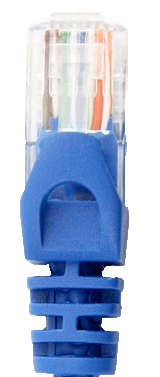
\includegraphics[angle=180,width=0.7cm]{img/plug.png}};
		\node[below] at (0.97,2) {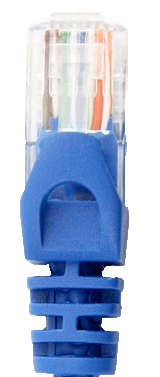
\includegraphics[angle=180,width=0.7cm]{img/plug.png}};
		%redraw
		\node at (0,-1.2) {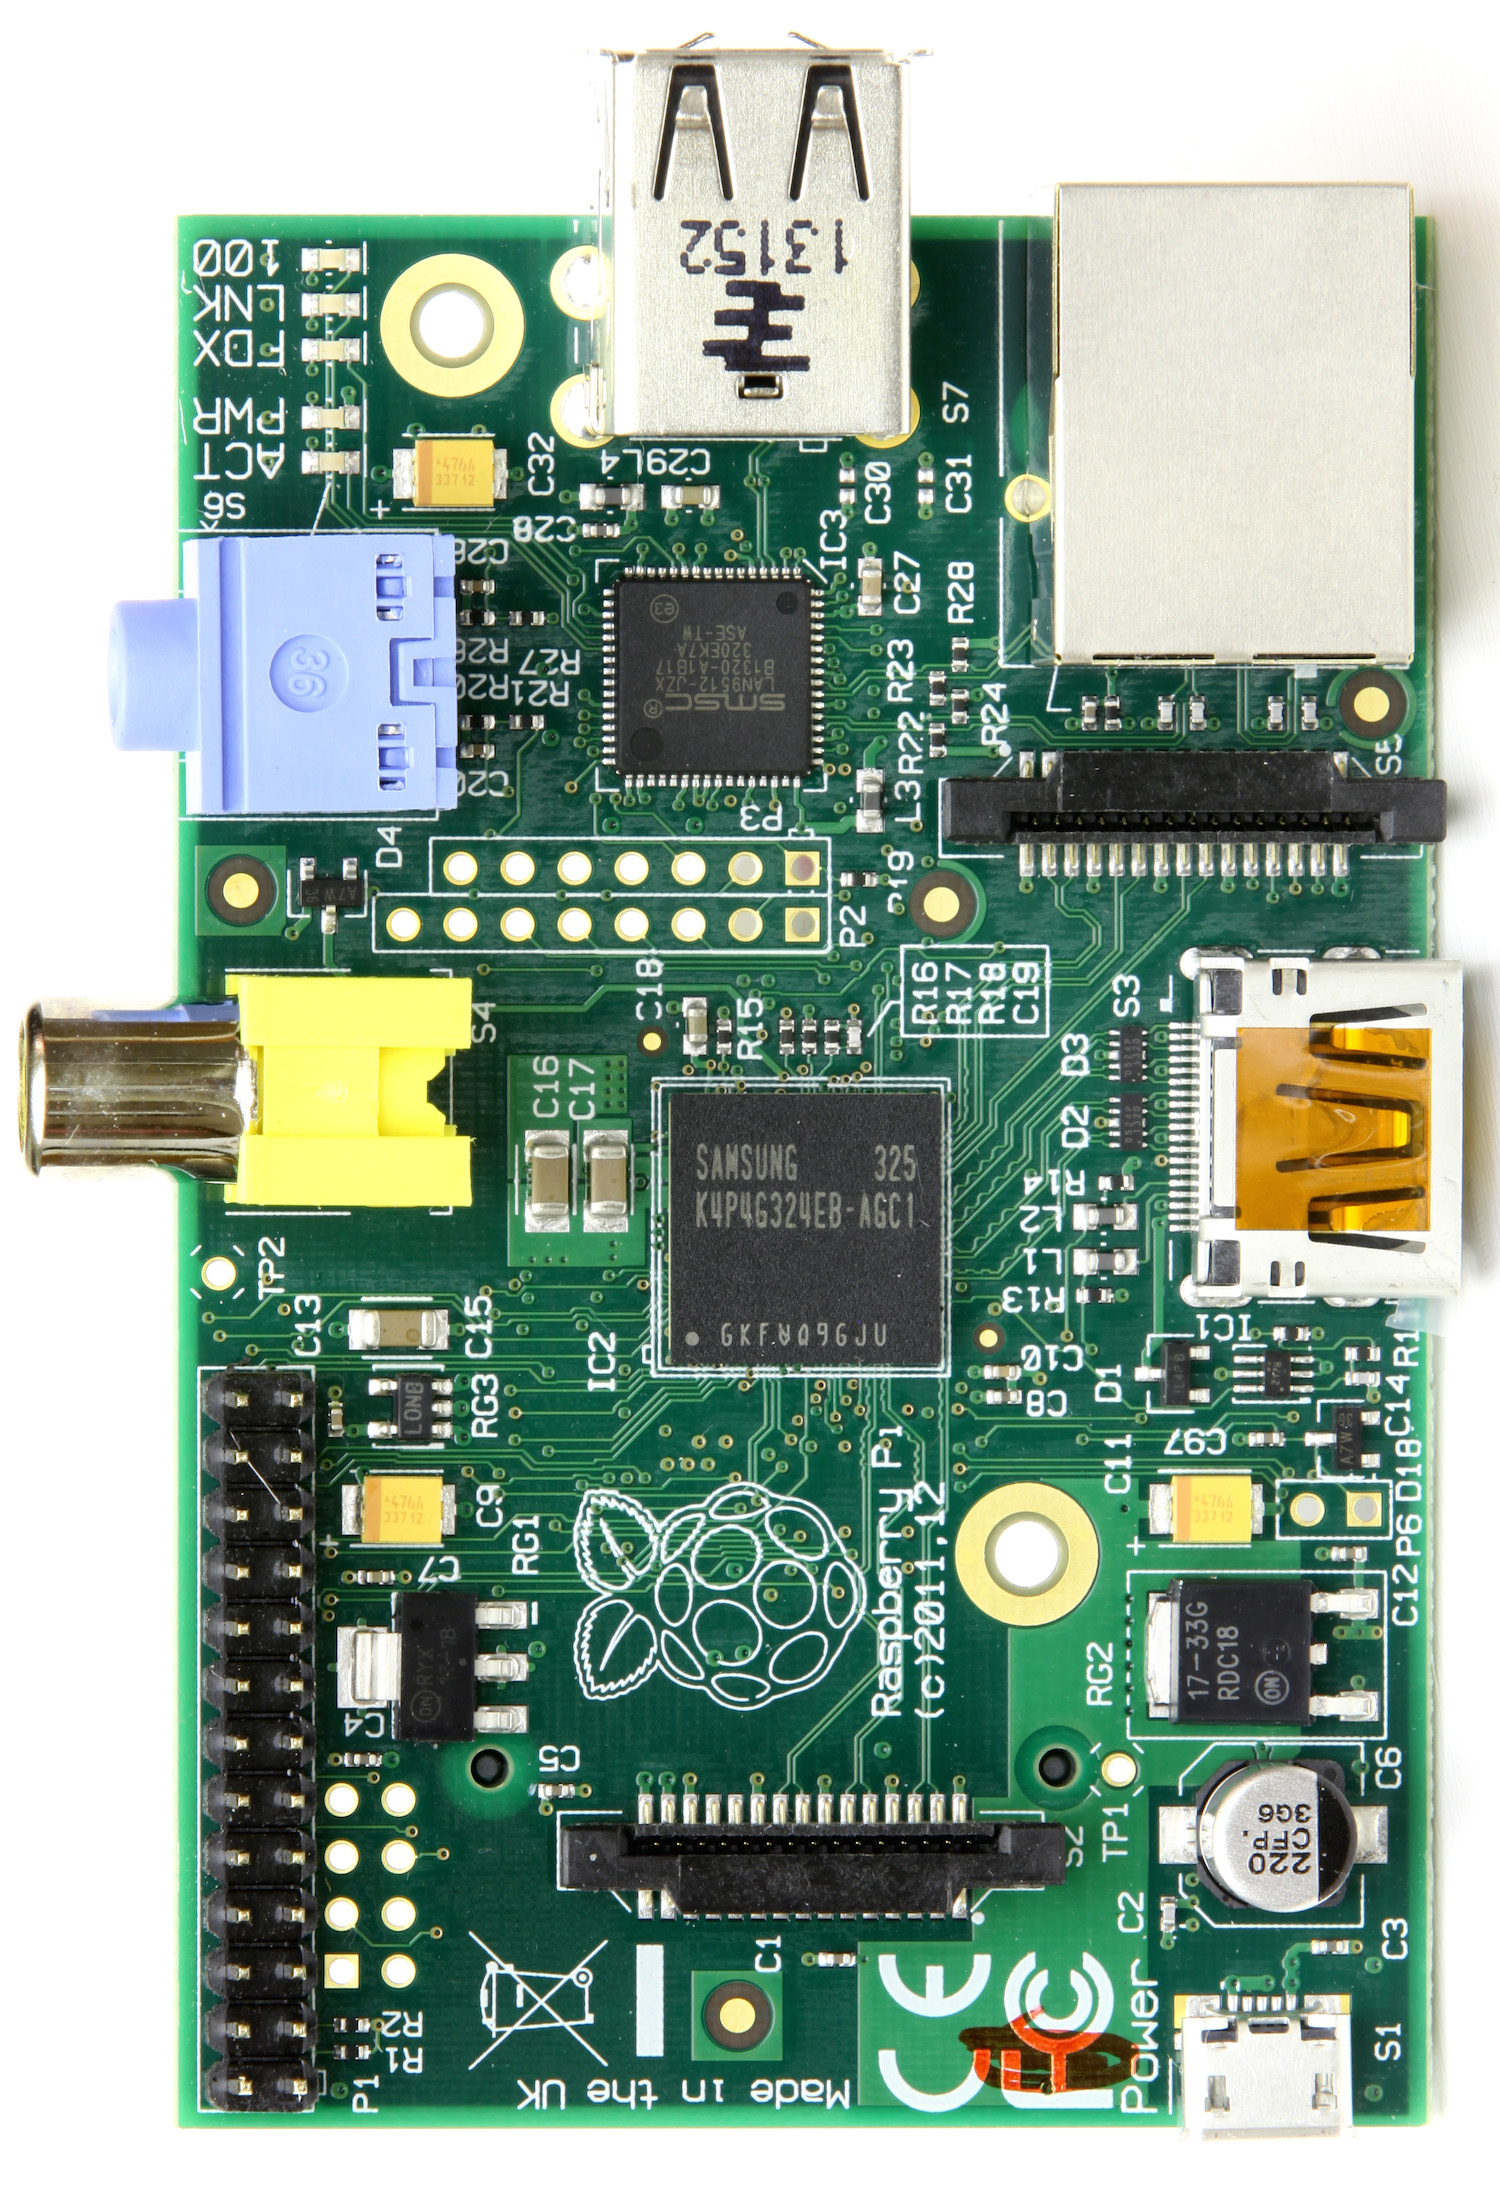
\includegraphics[width=3cm]{img/raspi.png}};
		\node at (-2.8,-3.3) {
\includegraphics[width=4cm]{img/music.png}};
		
		\draw (3,-2) rectangle node{Ethernet} +(2,0.5) 
			++(0,0.5) rectangle node{IP} +(2,0.5);
		\pause
		\draw (3,-1) rectangle node{UDP} +(2,0.5);
		\pause
		\draw (3,-0.5) rectangle node{rtpMIDI} +(2,0.5);
		\pause
		\fill[white] (2.9,-0.5) rectangle +(2.2,0.6);
		\draw (3,-0.5) -- +(2,0);
		\draw (2,-0.5) rectangle node{mDNS} +(2,0.5)
			++(2,0) rectangle node{rtpMIDI} +(2,0.5);
	\end{tikzpicture}
\end{frame}
\begin{frame}
	\centering
	\begin{tikzpicture}
		\node at (0,-1.2) {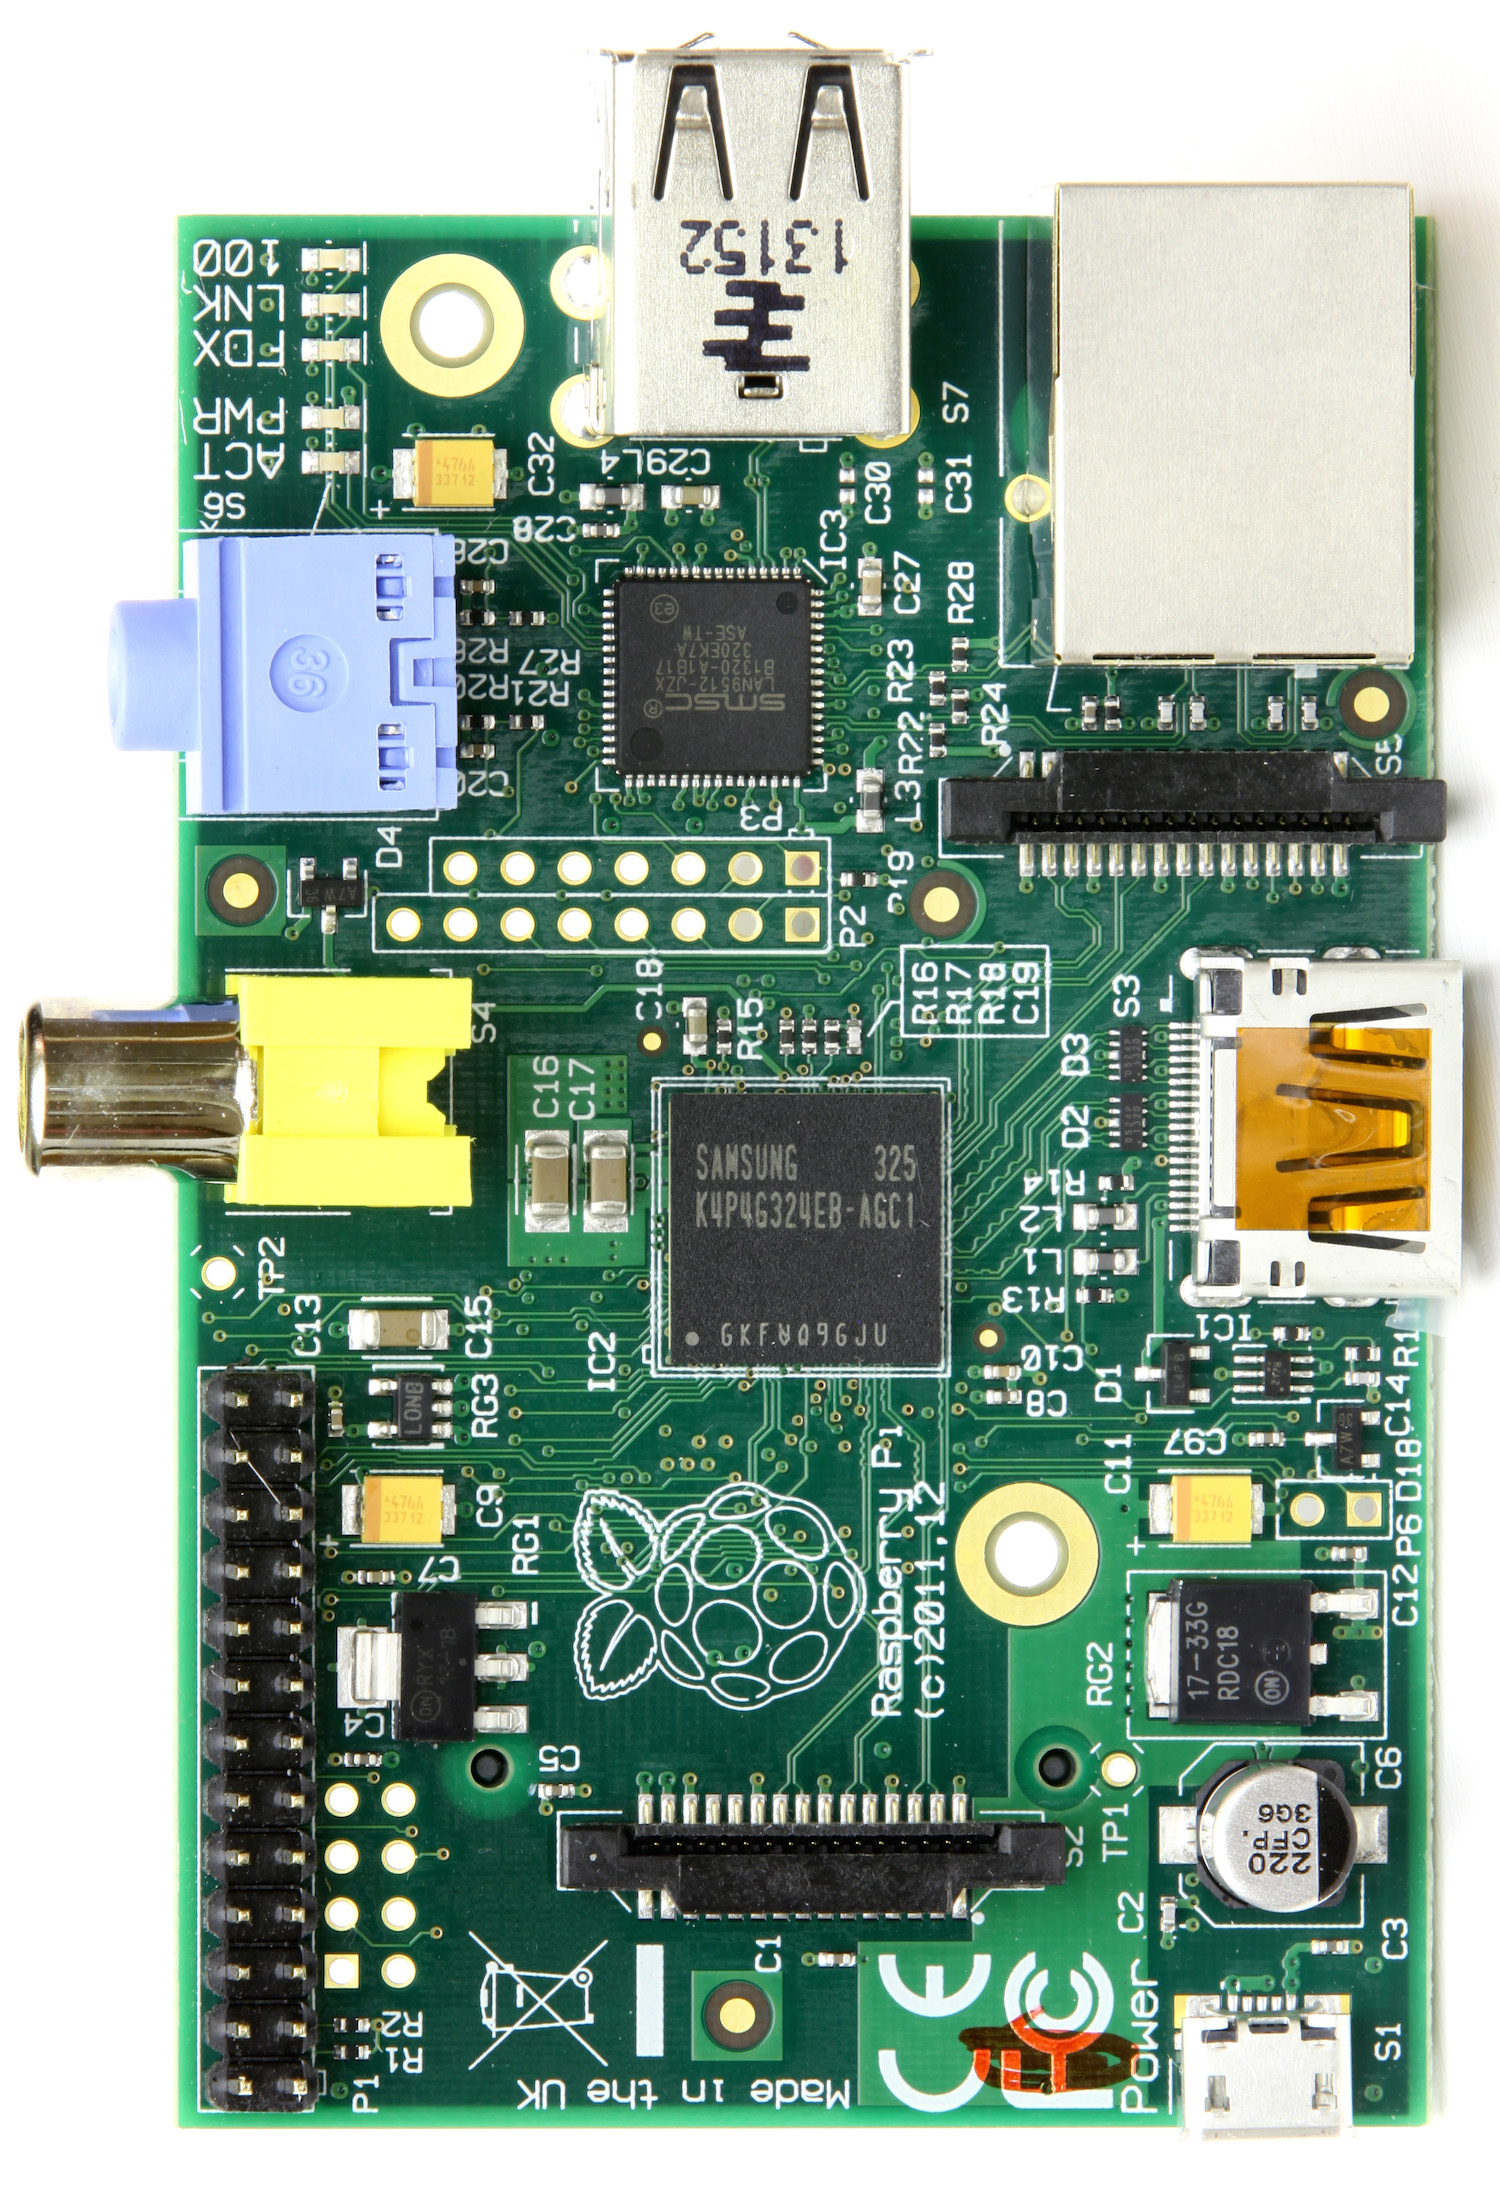
\includegraphics[width=3cm]{img/raspi.png}};
		\node at (-2.8,-3.3) {
\includegraphics[width=4cm]{img/music.png}};
		\draw[line width=0.6em,color=blue] (1,1.8) .. controls (1,3) and(4,3) .. (4,1.8);
		\node[below] at (3.97,2) {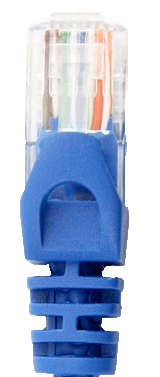
\includegraphics[angle=180,width=0.7cm]{img/plug.png}};
		\node[below] at (0.97,2) {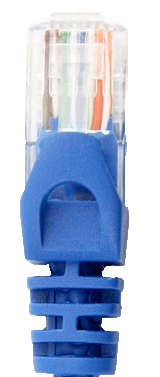
\includegraphics[angle=180,width=0.7cm]{img/plug.png}};
		%redraw
		\node at (0,-1.2) {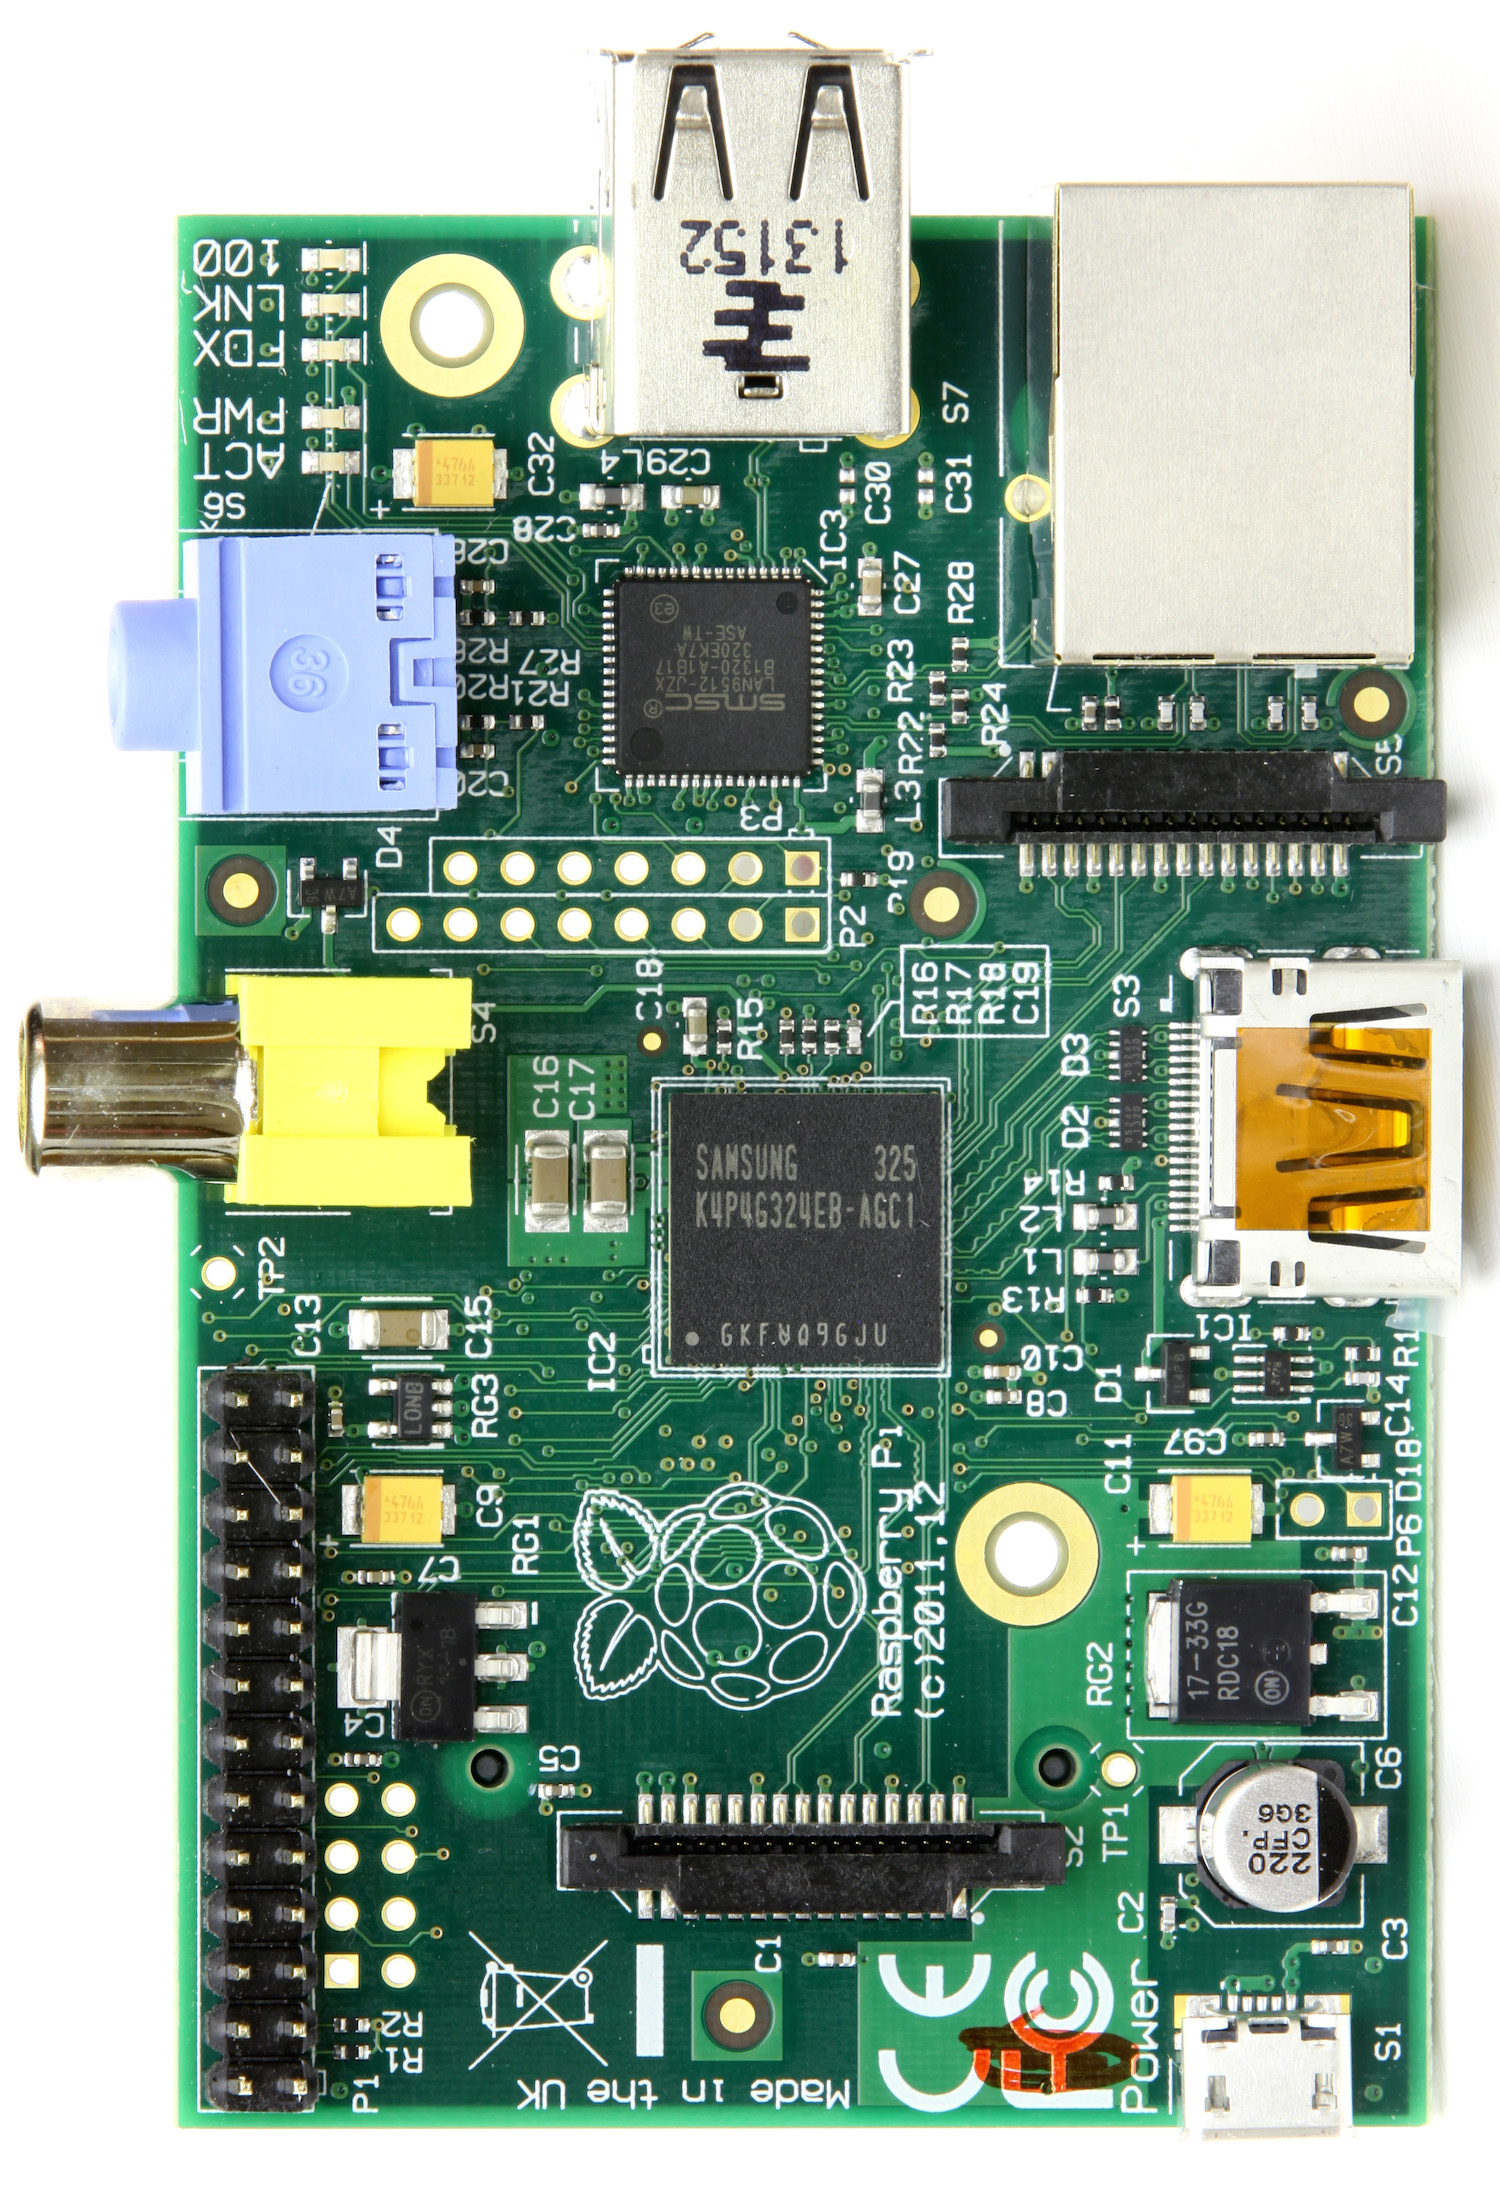
\includegraphics[width=3cm]{img/raspi.png}};
		\node at (-2.8,-3.3) {
\includegraphics[width=4cm]{img/music.png}};
		
		\draw (3,-2.5) rectangle node{Ethernet} +(2,0.5) 
			++(0,0.5) rectangle node{IP} +(2,0.5);
		\draw (3,-1.5) rectangle node{UDP} +(2,0.5);
		\draw (3,-1) rectangle node{SDP} +(2,0.5);
		\draw (2,-0.5) rectangle node{mDNS} +(2,0.5)
			++(2,0) rectangle node{rtpMIDI} +(2,0.5);
	\end{tikzpicture}
\end{frame}
\begin{frame}
	\centering
	\begin{tikzpicture}
		\node at (0,-1.2) {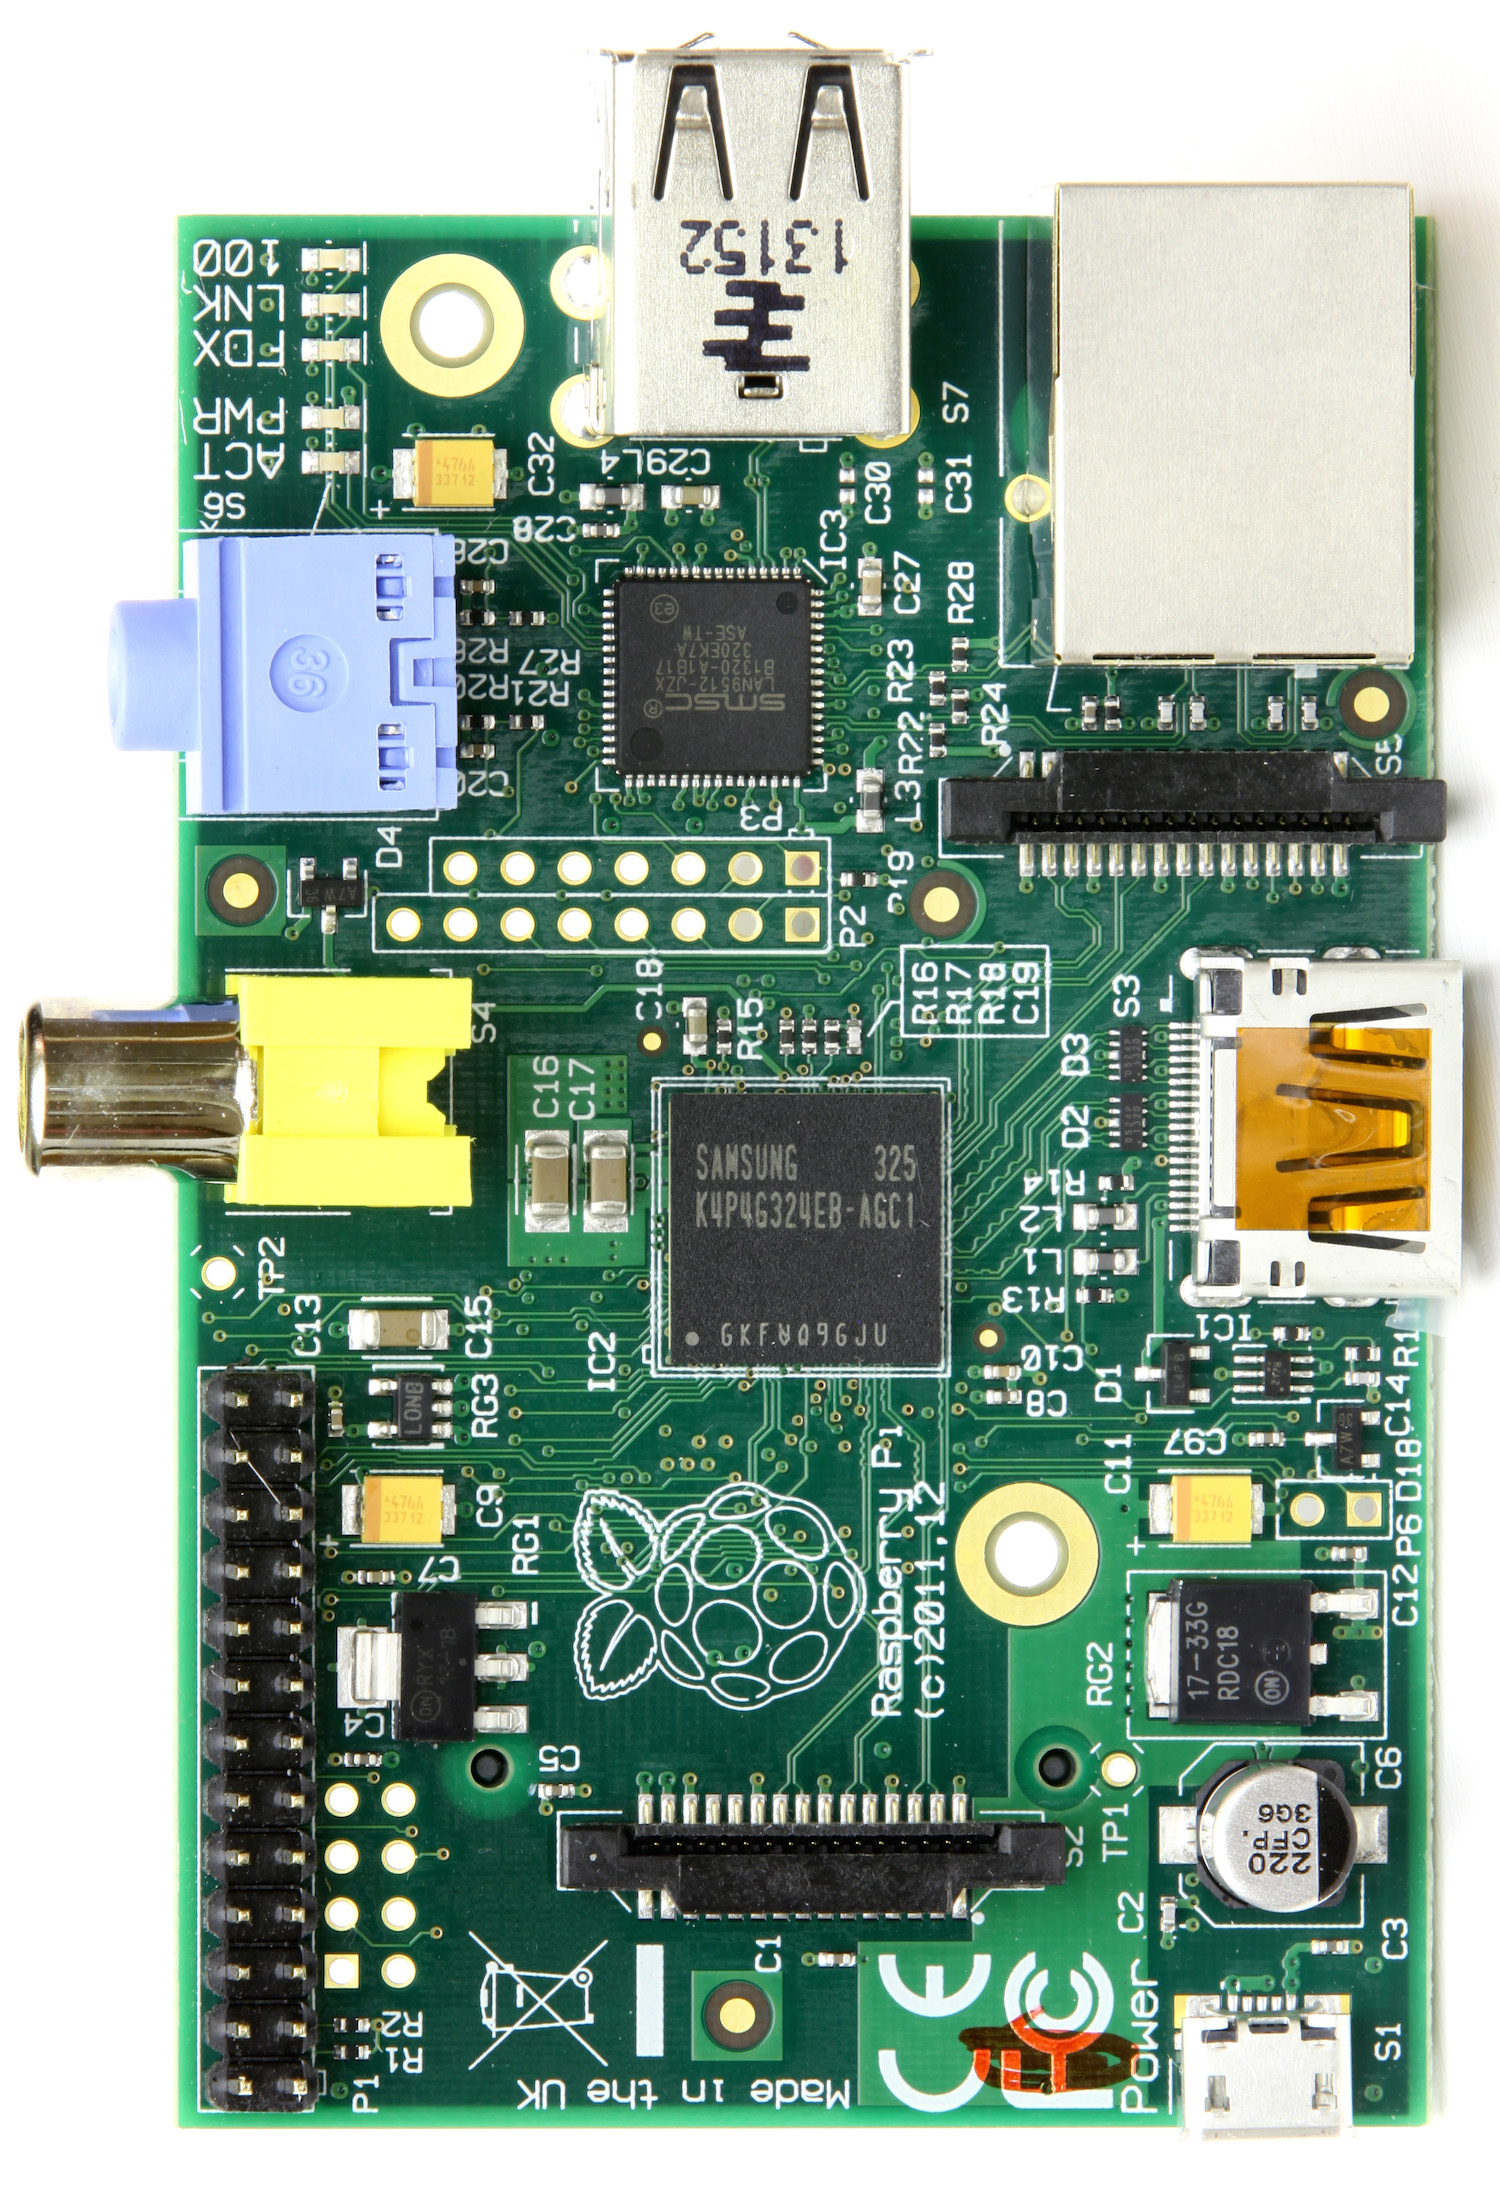
\includegraphics[width=3cm]{img/raspi.png}};
		\node at (-2.8,-3.3) {
\includegraphics[width=4cm]{img/music.png}};
		\draw[line width=0.6em,color=blue] (1,1.8) .. controls (1,3) and(4,3) .. (4,1.8);
		\node[below] at (3.97,2) {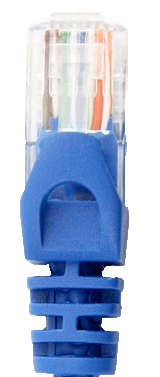
\includegraphics[angle=180,width=0.7cm]{img/plug.png}};
		\node[below] at (0.97,2) {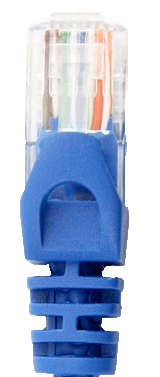
\includegraphics[angle=180,width=0.7cm]{img/plug.png}};
		%redraw
		\node at (0,-1.2) {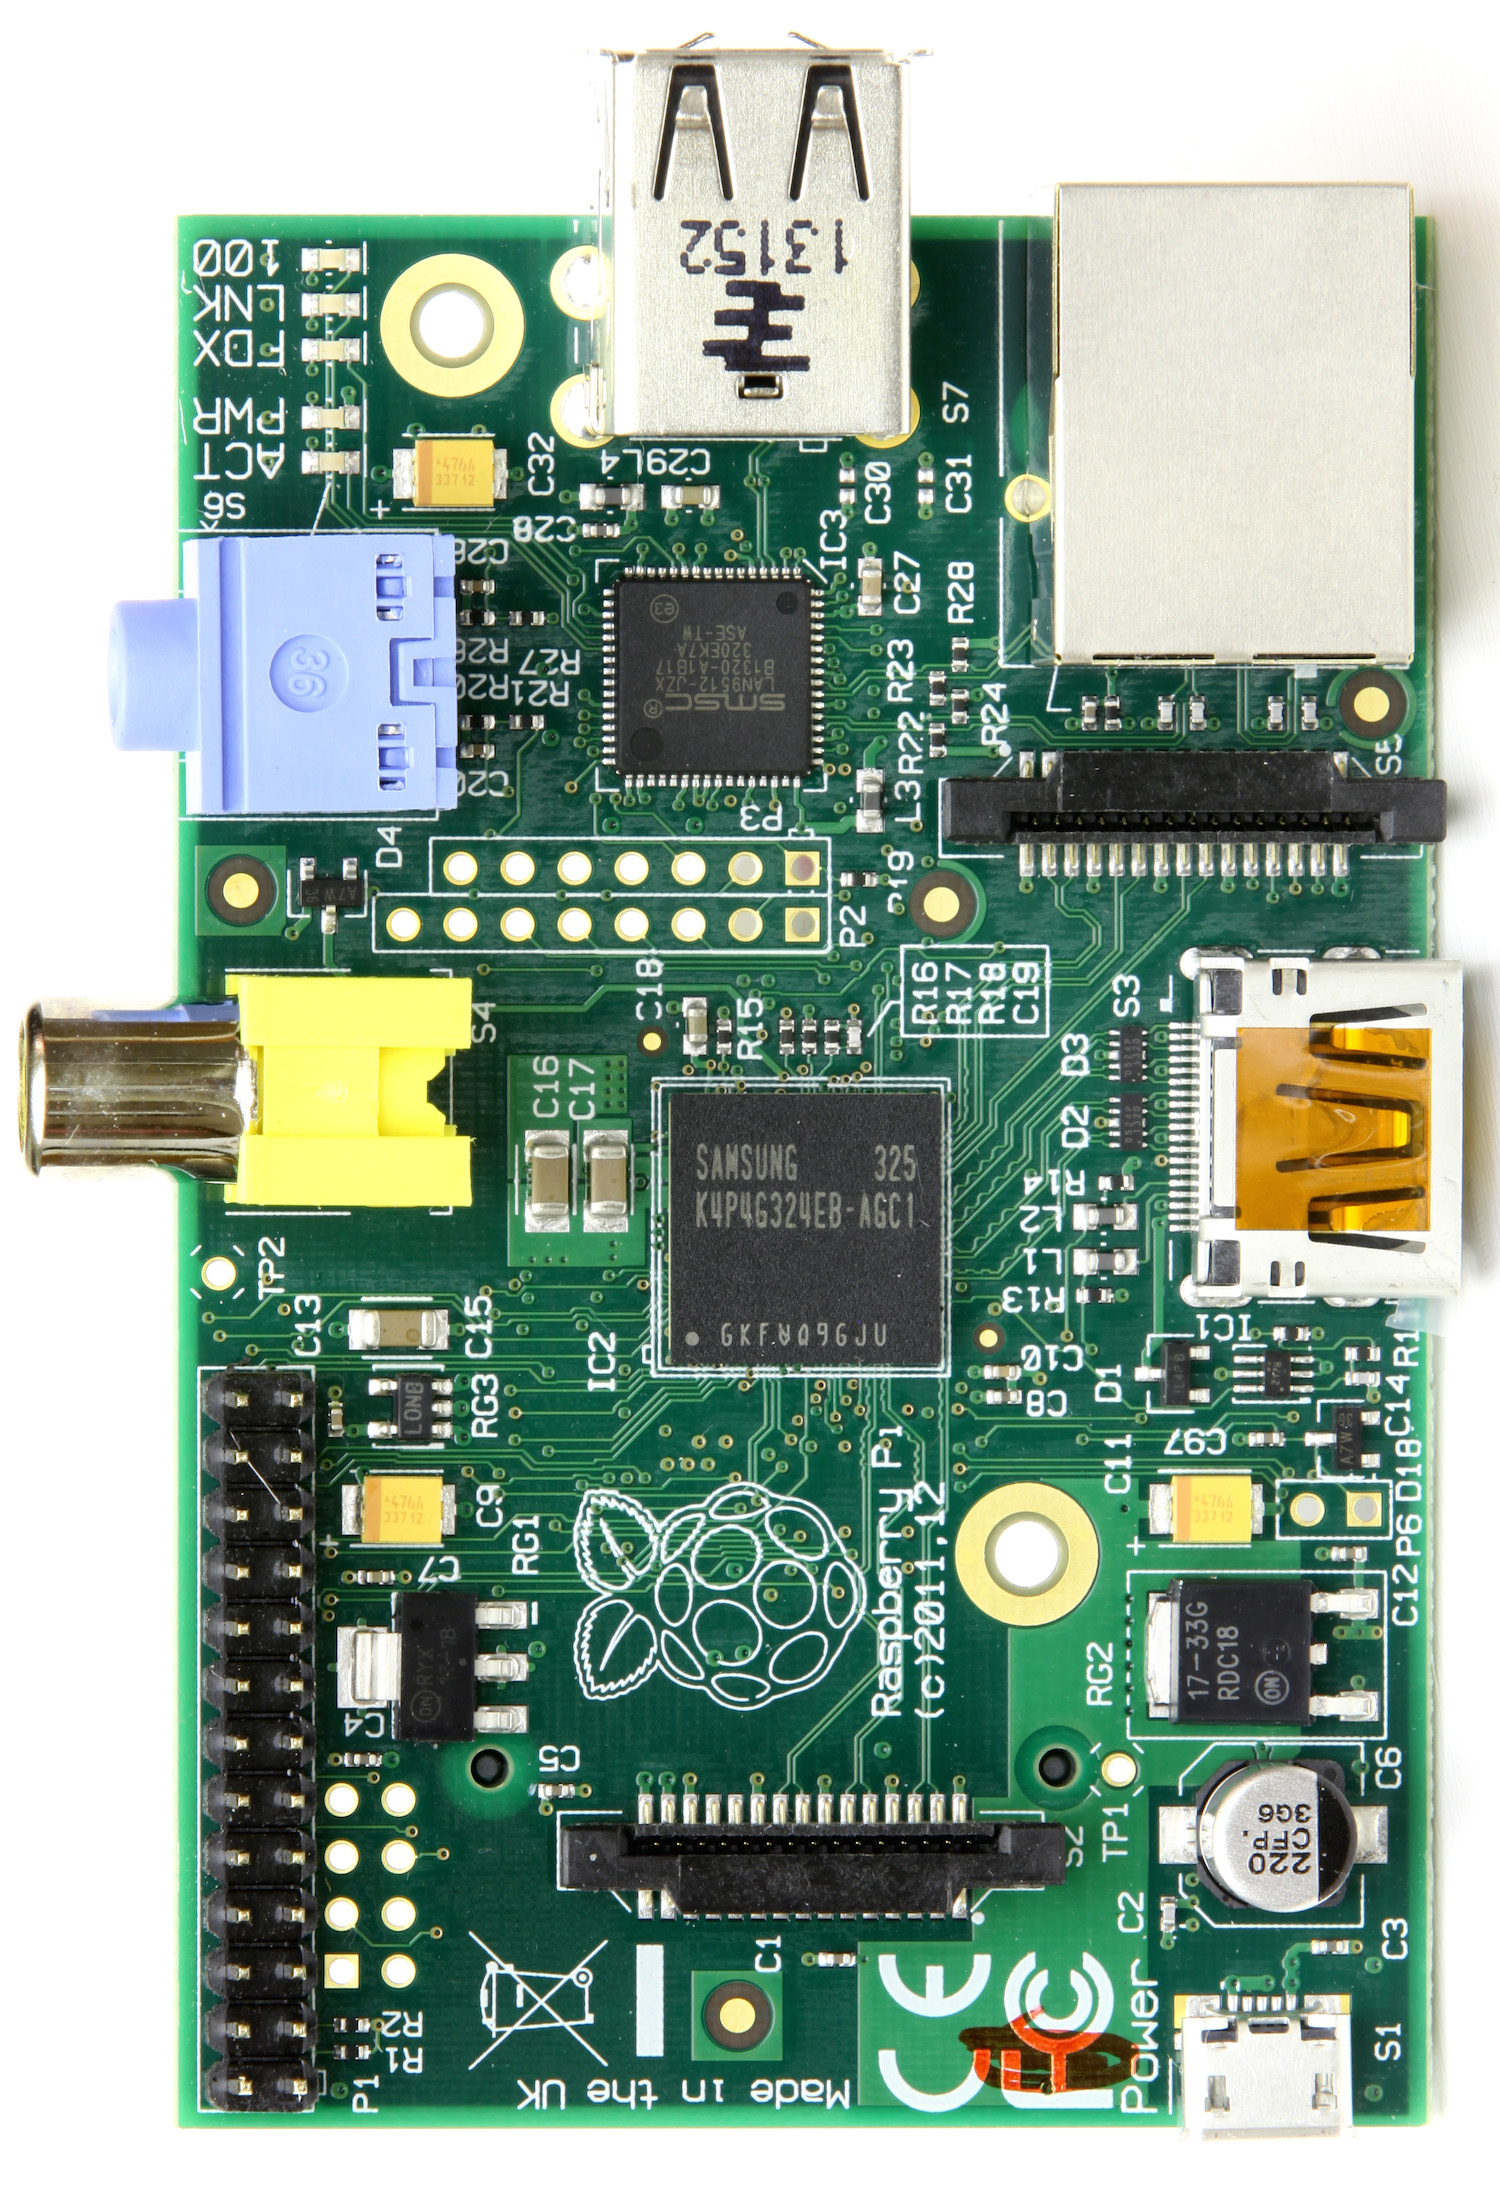
\includegraphics[width=3cm]{img/raspi.png}};
		\node at (-2.8,-3.3) {
\includegraphics[width=4cm]{img/music.png}};
		
		\draw (3,-2) rectangle node{Ethernet} +(2,0.5) 
			++(0,0.5) rectangle node{IP} +(2,0.5);
		\draw (3,-1) rectangle node{UDP} +(2,0.5);
		\draw (2,-0.5) rectangle node{Bonjour} +(2,0.5)
			++(2,0) rectangle node{appleMIDI} +(2,0.5);
	\end{tikzpicture}
\end{frame}
\begin{frame}{rtpMIDI}
	\begin{itemize}
		\item \st{RFC4695} RFC6295 
		\item reference snippets (UCB)
		\pause
		\item closed source
		\begin{itemize}
			\item Core MIDI Framework (OS X)
			\item Windows
			\item nmj (Java)\\$\vdots$
		\end{itemize}
	\end{itemize}
	\pause
	\centering
	
\includegraphics[width=4cm]{img/Node.pdf}
\end{frame}



\begin{frame}
	\centering
	\begin{tikzpicture}
		\node at (0,0.5) {
\includegraphics[width=6cm]{img/snail_n.jpg}};
		\node at (4,3) {\huge Real-Time};
		\node at (3.5,4) {\Large Latenz};
		\node at (5,2.3) {\large Performance (RPi)};
	\end{tikzpicture}
	
\end{frame}

%\begin{frame}[fragile]{ALSA $\Leftrightarrow$ rtpMIDI}
%	userspace APIs FTW!
%	
%
%\begin{lstlisting}
%input = new midi.input(),
%output = new midi.output(),
%session = ...createSession({
%    localName: 'Session 1',
%    bonjourName: 'Node RTPMidi',
%    port: 5008
%});
%input.on('message', function(deltaTime, msg) {
%    session.sendMessage(deltaTime, msg);
%});
%\end{lstlisting}
%
%\end{frame}

\begin{frame}{Setup}
	\begin{center}
	\begin{tikzpicture}
		\node at (1,0) {
\includegraphics[width=0.7cm]{img/apple.jpg}};
		\node (ssho) at (2,0) {\texttt{ssh}};
		\node (lano) at (4,0) {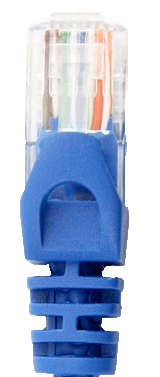
\includegraphics[width=0.5cm,angle=90]{img/plug.png}};
		\path[snake=expanding waves,segment length=1mm,segment angle=10,draw,thick] (ssho) -- (lano);
		\node at (5,-0.03) {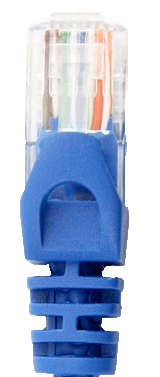
\includegraphics[width=0.5cm,angle=270]{img/plug.png}};
		\node at (6,0) {\texttt{ssh}};
		\node at (7,0) {user C};
	\end{tikzpicture}\\[0.1cm]
	
\begin{tikzpicture}
		\node at (0,0) {ALSA};
	\end{tikzpicture}\\[0.1cm]
	
	\begin{tikzpicture}
		\node (node) at (0.5,0) {
\includegraphics[width=1.5cm]{img/Node.pdf}};
		\node (rtp) at (2,0) {rtpMIDI};
		\node  at (3.5,0) {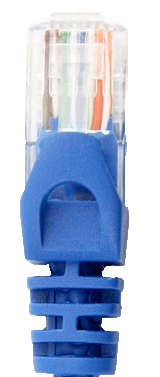
\includegraphics[width=0.5cm,angle=90]{img/plug.png}};
		
		\node (lan) at (4.5,-0.03) {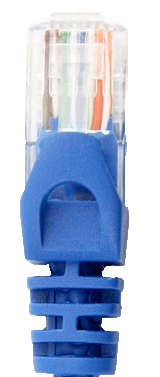
\includegraphics[width=0.5cm,angle=270]{img/plug.png}};
		
		\node (core) at (6.5,0) {
\includegraphics[width=0.5cm]{img/apple.jpg}};
		\node at (7.2,0) {MIDI};
		
		
		\path[snake=expanding waves,segment length=1mm,segment angle=10,draw,thick] (lan) -- (core);
		\node (ssho) at (8.5,0) {synth};
	\end{tikzpicture}\\[0.2cm]
	\end{center}
	
	ping (RTT)
	
	\[2.291\pm0.722\text{\,ms}\]
	
\end{frame}

\begin{frame}{Roundtrip}
	\begin{tikzpicture}
		\node [right] at (0,0) {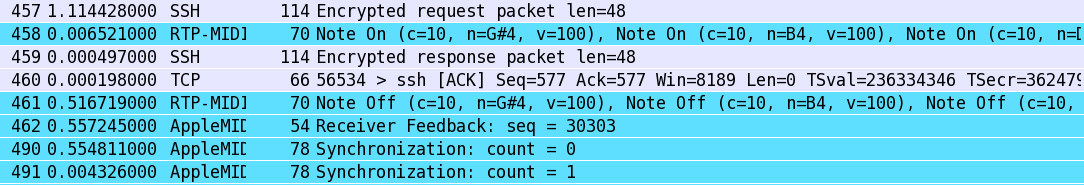
\includegraphics[height=4cm]{img/wire.jpg}};
		\pause
		\node at (2.5,2.5) {$\Delta t$ [s]};
	
		%\draw (1.1,1.05) rectangle (3.6,1.5);
		\fill[opacity=0.7,fill=white] (0,-2.2) -- (0,2.2) -- (1.1,2.2) -- (1.1,1.05) -- (3.6,1.05) -- (3.6,1.5) -- (1.1,1.5) -- (1.1,2.2) -- (14,2.2) -- (14,-2.2) -- cycle;
	\end{tikzpicture}
	
	\[\approx 7\pm2\text{\,ms}\]
	
\end{frame}

\begin{frame}{Development}
	\begin{itemize}
		\item rtpMIDI protocol implementation 
		\item in kernel space
		\pause
		\item called by GPIO ISRs
	\end{itemize}
\end{frame}

\begin{frame}{TODO}
	\begin{itemize}
		\item Jitter
		\item Ausreißer
		\item Journal/ever playing note
		\item Kapazität
		\item support multiple keys
		\item easy configuration of GPIO layout
		\item optional: support for different music devices
	\end{itemize}
\end{frame}

\begin{frame}
	\centering
	\Huge Demo
\end{frame}
